\documentclass[a4paper, utf8]{ctexart}
\usepackage[fontset=Fandol]{ctex}
\usepackage{anyfontsize}
\usepackage{algorithm}
\usepackage{longtable}
\usepackage{abstract}
\usepackage{amsfonts}
\usepackage{appendix}
\usepackage{booktabs}
\usepackage{enumitem}
\usepackage{fancyhdr}
\usepackage{geometry}
\usepackage{graphicx}
\usepackage{tabularx}
\usepackage{listings}
\usepackage{amsmath}
\usepackage{caption}
\usepackage{lipsum}
\usepackage{minted}
\usepackage{xcolor}
\usepackage{array}

\geometry{a4paper,left=31mm,right=31mm,top=25mm,bottom=25mm}
\CTEXsetup[format={\Large \bfseries}]{section}

\setlength{\parindent}{2em}
\pagestyle{fancy}
\fancyhf{}
\fancyhead[L]{并行程序设计与算法实验\ 实验报告}
\fancyhead[R]{Lab8\ 并行多源最短路径搜索}
\fancyhead[C]{}
\fancyfoot[C]{\thepage}
\fancyfoot[L,R]{}

\setCJKfamilyfont{zhsong}[AutoFakeBold = {2.17}]{SimSun}
\renewcommand*{\songti}{\CJKfamily{zhsong}}
\definecolor{LightGray}{gray}{0.9}

\title{\songti \bfseries Lab8\ 并行多源最短路径搜索}
\author{\fangsong 21307210\ \ 傅祉珏}
\date{\fangsong 中山大学计算机学院\ 广东广州\ 510006}

\begin{document}
	
	\begin{titlepage}
		\centering
		\rule{\textwidth}{1pt}
		\vspace{0.02\textheight}
		
		{\LARGE \kaishu 并行程序设计与算法实验\ 实验报告}
		
		\vspace{0.02\textheight}
		
		{\Huge \songti \bfseries Lab8\ 并行多源最短路径搜索}
		
		\vspace{0.025\textheight}
		\rule{0.83\textwidth}{0.4pt}
		\vspace{0.05\textheight} 
		\begin{figure}[htbp]
			\centering
			
\includegraphics[width=8cm, height=8cm]{./figure/计院院徽.jpg}
		\end{figure}
		
		\vspace{0.04\textheight} 
		{\Large 姓名:傅祉珏}
		
		\vspace{0.025\textheight} 
		{\Large 学号:21307210}
		
		\vspace{0.025\textheight} 
		{\Large 专业:计算机科学与技术}
		
		\vspace{0.025\textheight} 
		{\Large Email:futk@mail2.sysu.edu.cn}
		
		\vspace{0.025\textheight} 
		{\Large 完成时间:\today}
		
		\vspace{0.05\textheight} 
		\vfill
		
		{\large \today}
		\vspace{0.1\textheight}
		\rule{\textwidth}{1pt}
	\end{titlepage}
	\let\cleardoublepage\clearpage
	
	\maketitle
	
	\renewcommand{\abstractname}{\large \textbf{摘要}}
	\begin{abstract}
		本实验围绕无向图上的多源最短路径搜索(Multi-Source Shortest Path, MSSP)问题,探索并行计算在图算法中的应用,采用 OpenMP 框架实现了对多个源点的 Dijkstra 算法并行处理。图结构通过邻接表构建,测试数据中每一对点对均需计算其最短路径距离。实验重点评估在不同线程数(116)和图规模下,程序性能的变化与可扩展性。结果显示,随着线程数的增加,运行时间显著下降,在 68 线程时达到性能最优;但当线程数进一步增大至 16 时,反而因线程管理与资源争用开销导致性能退化。实验验证了任务级并行在图搜索中的有效性,也揭示了并行编程中的瓶颈问题,为后续扩展至更高并发度或分布式环境(如 MPI)提供了实践基础与启示。
		
		\noindent{\textbf{\heiti 关键词:}多源最短路径,OpenMP,并行计算,Dijkstra,线程调度。}
	\end{abstract}
	
	\section{实验目的}
	
	本实验旨在通过实现无向图上的多源最短路径搜索(Multi-Source Shortest Path, MSSP)问题,探索并行计算在图算法中的实际应用。实验使用 OpenMP、Pthreads 或 MPI 等任意一种并行编程框架,对 MSSP 问题进行并行化处理,并在不同线程(或进程)数量和图结构数据条件下,评估程序的性能表现。通过实验可进一步掌握并行编程模型的基本使用方法,理解多线程或多进程调度机制,以及将串行图算法转化为并行算法以提升计算效率的基本思路。
	
	图结构采用邻接表进行表示,输入包括边信息和测试点对信息,所有边视为无向边。在实验过程中需完成任意顶点对之间最短路径距离的计算,并输出测试点对对应的最短路径结果及整体计算所耗时间。通过对比不同线程数量(例如 1 至 16)下的运行性能,并结合图的规模(如顶点数量、平均度数等),分析并行算法的可扩展性、负载均衡性及其在大规模图处理任务中的适用性。
	
	\section{实验过程}
	
	本实验基于邻接表输入格式,使用 OpenMP 框架实现了无向图上的并行多源最短路径搜索算法。整个实验流程可分为图数据读取与构建、测试数据处理、路径搜索的并行实现、以及性能测试与结果输出四个主要阶段。
	
	首先,在图数据读取阶段,程序从指定的邻接表文件中读取图的结构信息。每一行包含两个顶点编号以及它们之间的边权重。考虑到图为无向图的性质,在邻接表中对每条边都进行了双向插入,即若存在一条从顶点 $u$ 到顶点 $v$ 的边,则邻接表中既记录 $u \rightarrow v$ 的边,也记录 $v \rightarrow u$ 的边,从而确保后续路径搜索时任意两个顶点之间的连通性信息是对称可用的。在读取过程中还同步更新图中最大顶点编号,以确保后续用于存储最短路径的数组或向量可以覆盖所有节点编号。
	
	\begin{minted}[baselinestretch=1, framesep=0mm, escapeinside=||]{cpp}
void read_graph(const string& filename, unordered_map<int, vector<Edge>>& graph,
                int& max_node) {
    ifstream file(filename);
    string line;
    getline(file, line); // skip header

    int u, v;
    float w;
    max_node = 0;
    while (getline(file, line)) {
        stringstream ss(line);
        string token;
        getline(ss, token, ','); if (token.empty()) continue;
        u = stoi(token);
        getline(ss, token, ',');
        v = stoi(token);
        getline(ss, token, ',');
        w = stof(token);

        graph[u].push_back({v, w});
        graph[v].push_back({u, w}); // undirected
        max_node = max(max_node, max(u, v));
    }
}
	\end{minted}
	
	随后程序处理测试数据文件,从中提取所有待评估的顶点对,并构建对应的源点集合。测试数据中每一行列出了一个源点和一个目标点,要求输出这两个点之间的最短路径距离。通过对测试文件的遍历,提取所有唯一的源点编号并组成源点集合,用于后续的多源最短路径计算。此外,程序还根据测试数据中出现的最大节点编号,与图结构中出现的最大编号进行比较,取最大值作为整体图中节点编号的上界,从而统一数据结构的大小。
	
	\begin{minted}[baselinestretch=1, framesep=0mm, escapeinside=||]{cpp}
{
    ifstream tf(test_file);
    string line;
    getline(tf, line); // skip header

    while (getline(tf, line)) {
        stringstream ss(line);
        string token;
        int s, t;

        getline(ss, token, ','); if (token.empty()) continue;
        s = stoi(token);
        getline(ss, token, ','); t = stoi(token);
        // ignore third column (distance)

        test_pairs.emplace_back(s, t);
        source_set.insert(s);
        V2 = max(V2, max(s, t));
    }
}
    
int V = max(V1, V2);  // ensure vector size covers both graph + test data
vector<int> sources(source_set.begin(), source_set.end());
vector<vector<float>> all_dist(V + 1);
	\end{minted}
	
	在路径搜索阶段,实验采用 Dijkstra 算法作为单源最短路径计算的基础算法。Dijkstra 算法适用于非负权图,利用优先队列实现从源点出发的最短路径扩展。为实现多源并行搜索,程序将每一个源点的 Dijkstra 计算任务作为一个独立单元,并通过 OpenMP 的 \verb|parallel for| 并行循环进行调度和执行。线程数量通过程序参数灵活指定(例如设置为 1、2、4、8、16 等),并通过 \verb|num_threads| 控制实际运行时所使用的线程数量,从而可以在不同并行度条件下进行实验对比。
	
	\begin{minted}[baselinestretch=1, framesep=0mm, escapeinside=||]{cpp}
vector<float> dijkstra(int src, const unordered_map<int, vector<Edge>>& graph,
                       int V) {
    vector<float> dist(V + 1, INF);
    priority_queue<pair<float, int>, vector<pair<float, int>>, greater<>> pq;
    dist[src] = 0;
    pq.push({0, src});
    while (!pq.empty()) {
        auto [d, u] = pq.top(); pq.pop();
        if (d > dist[u]) continue;
        if (graph.count(u) == 0) continue;
        for (auto& edge : graph.at(u)) {
            if (dist[edge.to] > dist[u] + edge.weight) {
                dist[edge.to] = dist[u] + edge.weight;
                pq.push({dist[edge.to], edge.to});
            }
        }
    }
    return dist;
}
	\end{minted}
	
	为了提升线程执行效率并缓解任务不均衡的问题,OpenMP 并行循环采用了 dynamic 调度策略。由于图结构可能存在稀疏与稠密混合的情况,某些源点的搜索路径可能较短,某些则可能涉及大量节点,通过动态调度能够更好地分配计算资源,减少线程空闲和等待时间。每个线程在完成一个源点的 Dijkstra 搜索后,将结果存入全局的距离结果数组 \verb|all_dist| 中,供后续路径查询使用。
	
	\begin{minted}[baselinestretch=1, framesep=0mm, escapeinside=||]{cpp}
double start = omp_get_wtime();

#pragma omp parallel for num_threads(num_threads) schedule(dynamic)
for (int i = 0; i < sources.size(); ++i) {
    int s = sources[i];
    vector<float> dist = dijkstra(s, graph, V);
    all_dist[s] = dist;
}

double end = omp_get_wtime();
cout << "Time taken: " << (end - start) * 1000 << " ms\n";
	\end{minted}
	
	实验最后统计并输出整个并行计算阶段的执行耗时(以毫秒为单位),为后续的性能分析提供量化依据。此外,尽管主程序中用于输出所有测试点对的最短路径结果的部分被注释,为实验的完整性保留了输出逻辑,可在需要时启用以验证正确性。通过在不同规模图数据和不同线程数量下反复测试,可以评估并行算法的加速效果、可扩展性和适用性。
	
	\section{实验结果}
	
	为了评估并行多源最短路径搜索算法在不同线程数量下的性能表现,实验针对固定规模的数据集进行了 10 轮重复测试,并记录了从 1 到 16 个线程配置下的运行时间(单位:毫秒)。通过对各实验轮次的平均值进行分析,可以更直观地反映出并行度对算法执行效率的影响。
	
	\begin{figure}[htbp]
		\centering
		\begin{minipage}{.45\textwidth}
			\centering
			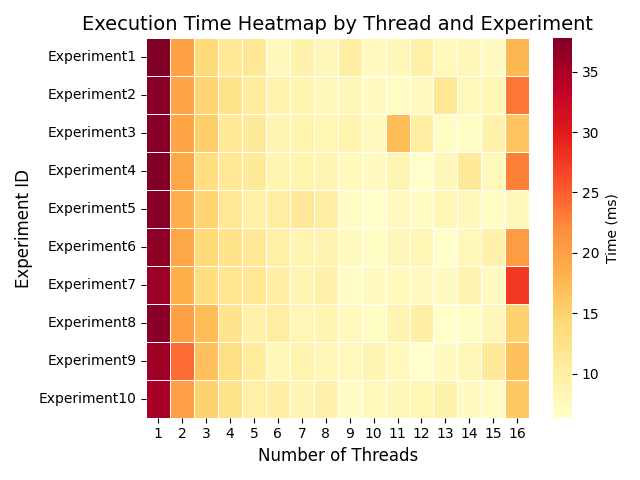
\includegraphics[width=.78\textwidth]{./figure/TimeHeatmap.png}
			\caption{运行时间热力图}
		\end{minipage}
		\begin{minipage}{.45\textwidth}
			\centering
			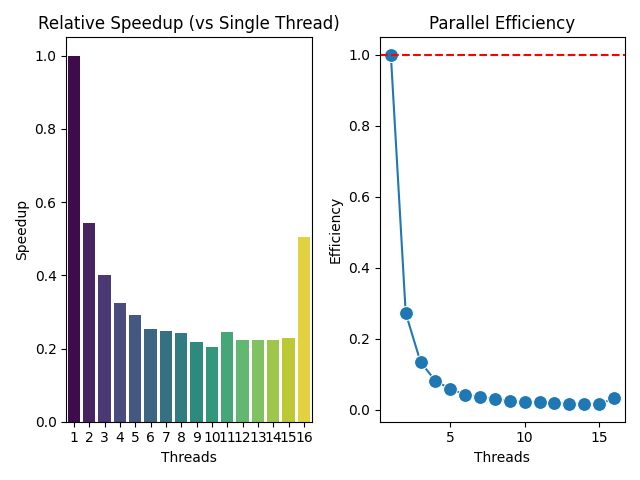
\includegraphics[width=.78\textwidth]{./figure/Speedup.png}
			\caption{加速比趋势对比图}
		\end{minipage}
	\end{figure}
	
	从实验结果来看,单线程执行时平均耗时约为 36.735 毫秒,作为串行基准。随着线程数量的增加,运行时间呈现明显下降趋势,2 线程时下降至约 19.977 毫秒,3 线程进一步降低至 14.764 毫秒,4 线程时为 11.897 毫秒,已经接近串行时长的三分之一,说明在初始并行化阶段,OpenMP 能够有效地将多源任务分发给多个线程并发处理,显著减少总计算时间。
	
	当线程数增至 6 到 8 时,平均运行时间进一步缩短至 9.322 毫秒(6 线程)和 8.878 毫秒(8 线程),此时加速比逐渐趋于平缓,开始出现性能提升边际递减的现象。随着线程数进一步增至 9、10、11、12,运行时间虽仍在波动下降(平均在 7.5~8.9 毫秒之间),但波动幅度开始加大,部分轮次出现了较为明显的波动,例如 11 线程的第三轮实验时间为 17.0986 毫秒,远高于其他轮次。
	
	特别值得注意的是,当线程数增加至 16 时,运行时间反而上升至平均 18.498 毫秒,明显劣于 8 线程配置。这表明过多线程反而引入了显著的线程管理开销、上下文切换成本和资源竞争,导致并行效率下降。这种现象在使用共享内存模型的 OpenMP 框架中较为常见,尤其当任务规模有限或计算密度不足以支撑更多线程时,更容易受到线程调度、缓存争用等系统瓶颈的影响。
	
	\begin{figure}[htbp]
		\centering
		\begin{minipage}{.45\textwidth}
			\centering
			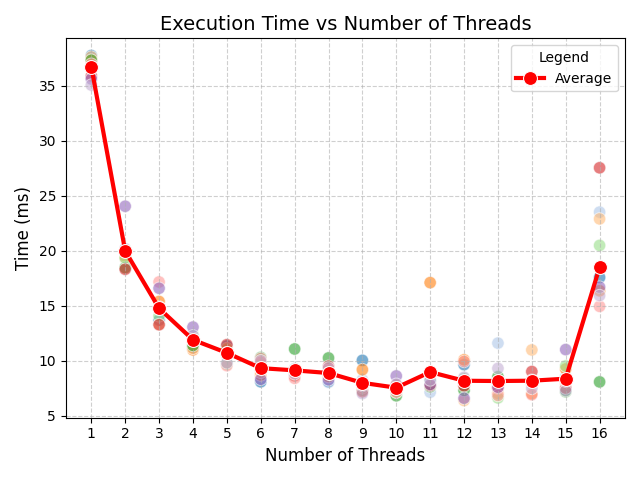
\includegraphics[width=.8\textwidth]{./figure/TimevsThreads.png}
			\caption{时间随线程增长趋势图}
		\end{minipage}
		\begin{minipage}{.45\textwidth}
			\centering
			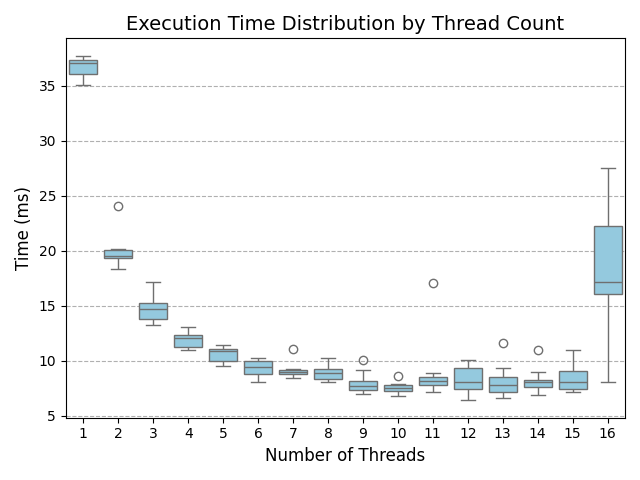
\includegraphics[width=.8\textwidth]{./figure/TimeDistribution.png}
			\caption{不同实验的运行时间分布}
		\end{minipage}
	\end{figure}
	
	综上所述,实验结果验证了并行化对于多源最短路径问题在一定线程数范围内可带来显著加速效果,最佳性能通常出现在 6 到 10 线程之间。在超过该范围后,线程之间的同步与资源竞争逐渐抵消了并行带来的计算优势。因此,在实际应用中,线程数量的选择应结合任务规模与计算平台特性进行调优,以实现最优性能和资源利用率。
	
	\section{总结与思考}
	
	\subsection{实验总结}
	
	本次实验围绕多源最短路径搜索问题,采用 OpenMP 框架实现了并行化处理,并通过大量实验验证了其在中小规模图数据集上的性能提升效果。实验过程中,我们构建了完整的数据处理流程,包括图数据的读取与建模、测试点对的提取、Dijkstra 算法的并行封装与执行、以及最终运行性能的定量评估。通过逐步增加线程数,我们观察到在 2 至 8 个线程范围内,算法运行时间随线程数增加显著下降,充分验证了任务级并行在多源路径搜索问题中的有效性。
	
	然而,实验也揭示了并行编程中的性能瓶颈与挑战。特别是在线程数超过 10 后,程序整体性能趋于不稳定,甚至在 16 线程配置下出现运行时间反弹,暴露出线程管理开销、资源争用与调度不均衡等问题。这些现象提示我们,在设计并行算法时,不应一味追求高并发度,而应依据问题本身的并行粒度、硬件平台的特性以及调度策略灵活调整线程数。此外,动态调度策略(schedule(dynamic))在处理具有任务长度差异的场景中展现了优越性,在一定程度上缓解了工作负载不均衡的问题。
	
	综合而言,本实验不仅验证了 OpenMP 在图计算中的可行性与局限性,也为日后从事更大规模图并行计算、进一步探索 MPI 或 GPU 等高性能计算框架打下了坚实的基础。
	
	\subsection{实验心得}
	
	通过本次 Lab8 实验,我对并行编程在图计算中的实际应用有了更深入的理解。多源最短路径问题虽然逻辑上可以通过多个单源路径搜索并行处理,但在实际实现中,如何合理划分任务、控制线程调度以及优化资源利用,都是影响性能表现的关键因素。
	
	实验中我使用 OpenMP 框架实现了并行处理,并在固定数据集下测试不同线程配置的性能变化。OpenMP 所基于的共享内存模型非常适合中小规模图的并行化,尤其是当图的节点数适中、任务粒度均衡时,能够通过 \verb|parallel for| 和 \verb|dynamic schedule| 实现较理想的并行加速。然而,实验也显示出:当线程数过多、图数据规模不足时,线程调度开销和内存带宽瓶颈会抵消并行带来的优势,甚至导致性能下降。
	
	更进一步地思考,图结构本身的特性对并行性能也有重要影响。比如,当图的节点数非常大时,每一次 Dijkstra 执行的计算量也相应增大,整体任务变“重”,此时并行化带来的收益更明显;而若图的平均度数较高,意味着每个节点连接的邻居更多,Dijkstra 中对每个节点的松弛操作数量上升,优先队列维护的成本增加,反而可能造成单次任务执行时间不均、线程间负载不平衡,从而影响整体并行效率。在这种情况下,动态调度策略显得尤为重要,可以有效缓解线程空闲与资源浪费的问题。
	
	此外,不同的并行编程模型对大规模图计算任务的适配性也存在差异。OpenMP 更适合单机、多核的共享内存架构,开发简单,适合中等规模数据;而如果图的节点数量和边数量大幅增加(如百万级以上),采用 MPI 等分布式内存模型则更具优势。MPI 能够将任务分散到多个进程乃至多台机器上,并通过显式消息传递完成数据交换,避免共享内存中的资源竞争问题,更利于扩展到超大规模并行计算。在这一实验的基础上,若进一步采用 MPI 对源点集合划分并分配给多个进程进行 Dijkstra 处理,则更容易突破单机资源瓶颈,显著提升整体可扩展性。
	
	\let\cleardoublepage\clearpage
	
	\begin{thebibliography}{99}  
		\bibitem{ref1} 彼得·S·帕切科,\ 马修·马伦塞克.\ 并行程序设计导论[M].\ 黄智濒,\ 肖晨\ 译.\ 原书第2版.\ 北京:机械工业出版社,\ 2024.
		\bibitem{ref2} 黄聃.\ 课件5[EB/OL].\ [2025-3-10].\ https://easyhpc.net/course/221/lesson/1416/material/3173.
		\bibitem{ref3} 黄聃.\ 课件6[EB/OL].\ [2025-3-10].\ https://easyhpc.net/course/221/lesson/1450/material/3182.
	\end{thebibliography}
	
\end{document}
